\section{Исследование и построение решения задачи}
\label{sec:Section3} \index{Section3}

\subsection{Устройство архитектуры системы процессор-память}

\subsubsection{Микроархитектура процессора}

    Современный ЦП (центральный процессор) представляет собой
    систему взаимосвязанных между собой процессорных ядер, не обязательно одинаковых.

    Исполнение инструкции современным процессорным ядром является многостадийным конвейером
    из различных блоков. В зависимости от исполняемой рабочей нагрузки утилизируются различные блоки
    процессора, поэтому скорость исполнения таковой рабочей нагрузки сильно зависит
    от её особенностей (типа) и особенностей исполнения таковых нагрузок на блоках процессора.

    В наиболее общем виде можно разбить конвейер исполнения инструкции на процессоре на несколько
    последовательных стадий:
    \begin{enumerate}
        \item Чтение инструкции из памяти;
        \item Декодирование прочитанной инструкции;
        \item Исполнение инструкции на вычислительных блоках;
        \item Чтение/запись в память при необходимости;
        \item Запись результата исполнения инструкции в регистры процессора.
    \end{enumerate}

    Чаще всего приведённые выше стадии дробятся на несколько более узконаправленных стадий, применяются
    дополнительные оптимизации для ускорения исполнения инструкций а также их распараллеливания
    (например, кеширование декодированных инструкций и предсказатель ветвлений). Наиболее
    актуальным примером являются ядра процессора с маханизмом спекулятивного (внеочередного) выполнения
    инструкций (Out-of-Order), в которых используется алгоритм Томасуло, позволяющий реализовать
    исполнение машинных инструкций не в порядке их следования в машинном коде, а в порядке
    готовности к выполнению, за счёт чего значительно увеличивается скорость исполнения инструкций.

    В типичной реализации OoO используется ROB (Re-order buffer), который представляет собой
    циклический буфер и накапливает инструкции для обеспечения возможности их переупорядочить.
    Обычно в ROB попадают не исходные машинные иструкции, а прошедшие через стадию переименование
    регистров для избавления от зависимостей по данным (для дополнительного распараллеливания
    инструкций).

    Наибольший интерес в данной работе представляет организация обращений ядра процессора в память,
    также затрагиваются аспекты, связанные с OoO исполнением. Схема современного конвейера показана на
    рис. \ref{cortexA77}.

    \begin{figure}[!h]
        \caption{Схема конвейера процессора Arm Cortex A77 \cite{CortexA77Docs}}
        \centering
        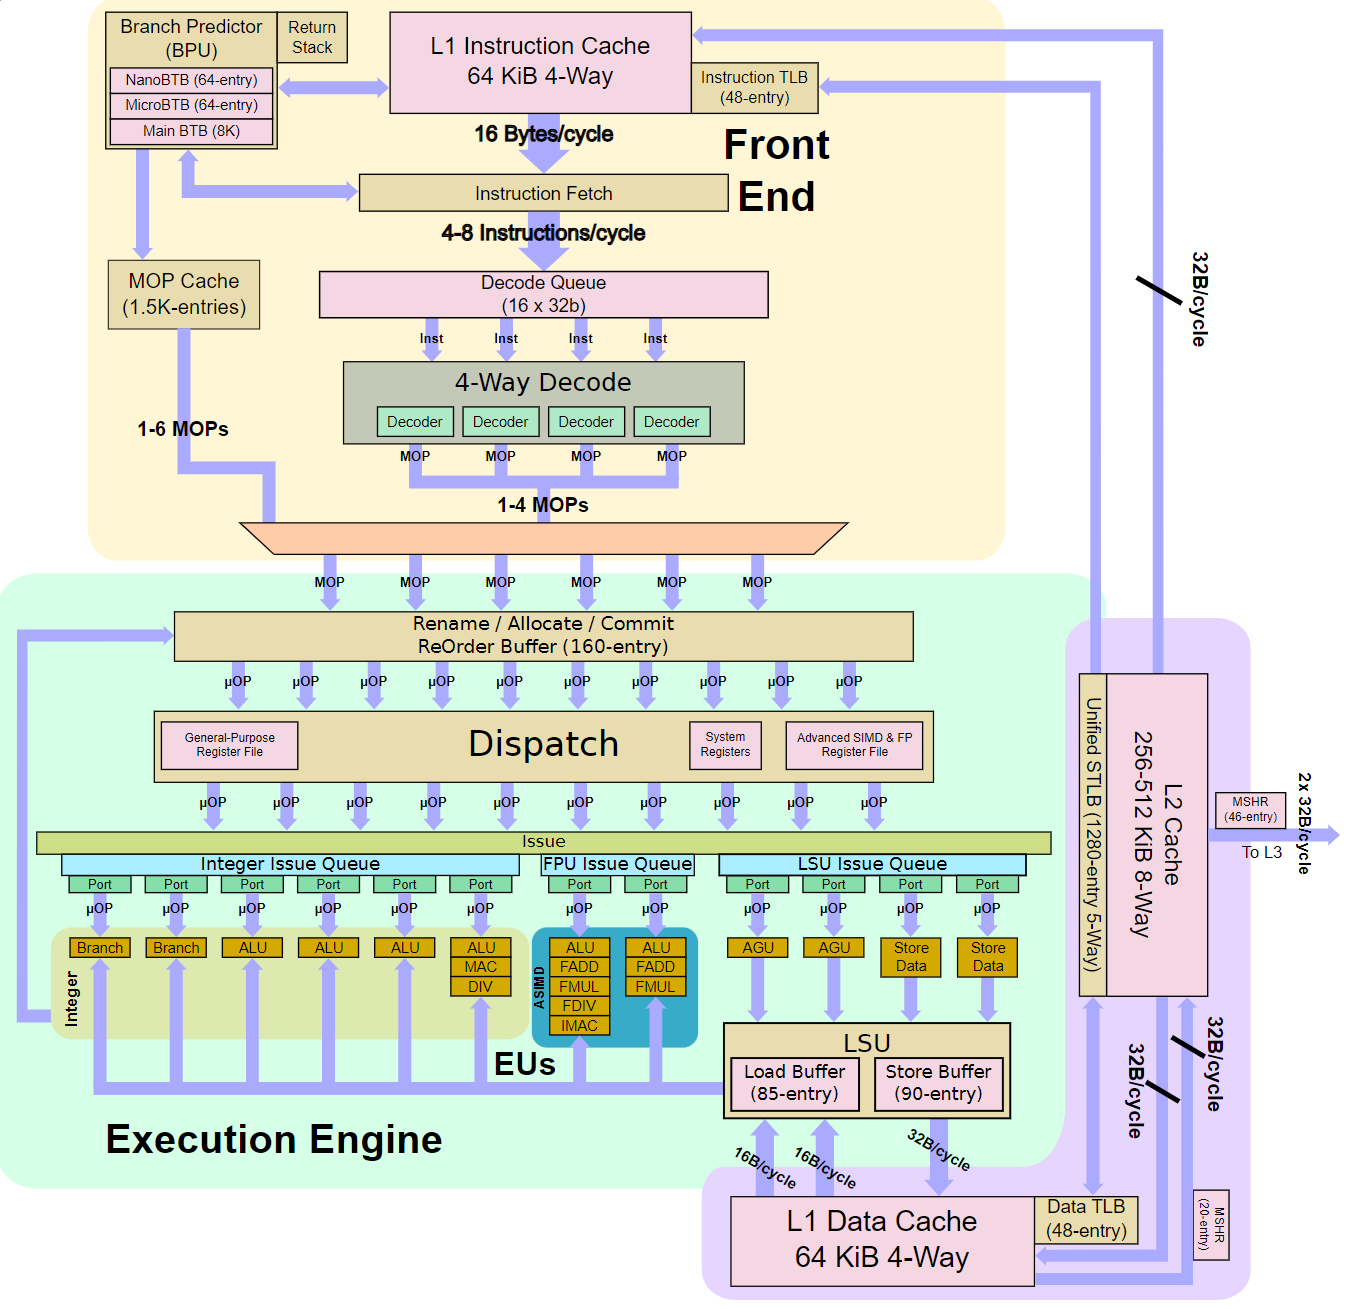
\includegraphics[width=161mm]{CortexA77}
        \label{cortexA77}
    \end{figure}

\subsubsection{Организация системы памяти}

    Процессор в современных мобильных системах встроен в так называемую SoC (System-on-chip --
    система на кристалле) систему -- электронная схема, которая выполняет цели компьютера
    и размещена на одной интегральной схеме. Таким образом, в такую систему встроены сразу процессор,
    таймеры, счётчики, интерфейсы для периферийных устройств, ОЗУ, ПЗУ и даже графический ускоритель.
    Именно таким образом устроены современные смартфоны, фотоаппараты, умные часы, элекронные книг
    и устройства схожего профиля.

    Одна из основных подсистем системы на кристалле -- подсистема памяти. Наиболее быстродействующими
    элементами памяти являются регистры ядра процессора, они же имеют наименьшее количество памяти,
    более высокую цену для производства и самую малую плотность расположения в электронной схеме.

    Учитывая малый объём возможного хранения данных с помощью регистров, а также
    что любая вычислительная система обладает локальностью (как по данным, так и по
    времени), почти всегда вводят дополнительные уровни памяти -- более дешёвые в производстве,
    имеющий больший объём и более высокую плотность ячеек хранения данных на электронной схеме.
    Более низкие уровни памяти являются кешами для более высоких.
    Таким образом, любая система имеет ОЗУ и кеши в качестве промежуточного хранилища данных
    (см. рис. \ref{CachePyramid}).

    Во всех современных мобильных системах в качестве ОЗУ используется LPDDR SDRAM
    (Low-Power Double Data Rate Synchronous Dynamic Random-Access Memory --
    динамическая оперативная память синхронного доступа с двойной скоростью передачи данных и
    с низким энергопотреблением). В дальнейшем для удобства будем использовать более простое
    обозначение для такой памяти -- DDR (Double Data Rate) память.

    Количество уровней кешей и объём их памяти напрямую зависят от требований к исполнению
    современных приложений и особенностей архитектуры мобильной системы,
    всегда являются компромиссом: с одной стороны, добавление дополнительного
    уровня кеша -- снижение вероятности обращения в DDR память (наиболее медленная память),
    а с другой -- введение постоянной дополнительной задержки при обращении в DDR, если данные
    в кешах отсутствуют.

    \begin{figure}[!h]
        \caption{Иерархия памяти в системе с 3-мя уровнями кешей}
        \centering
        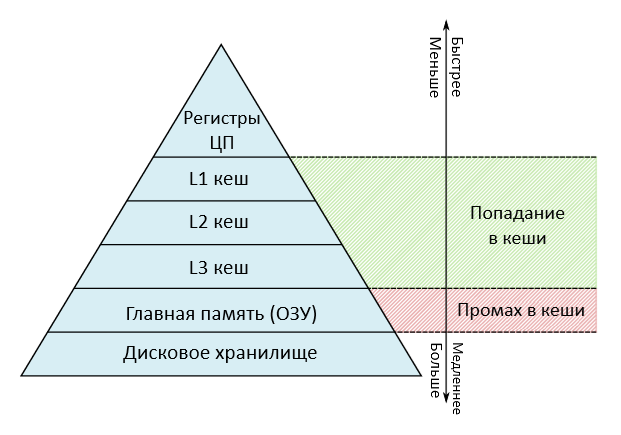
\includegraphics[width=116mm]{CachePyramidRU}
        \label{CachePyramid}
    \end{figure}

    Почти все современные процессоры имеют как минимум 2 уровня кешей. В системах на кристалле,
    как правило, последним (дополнительным) уровнем является системный кеш, который обычно
    не вносят в список уровней кешей процессора, так как он используется не только самим процессором,
    но также и различными периферийными устройствами, такими как графический ускоритель, ускоритель
    нейронных сетей и т.д.. Пример системы с 2-ся уровня кешей показан на рис. \ref{MulticoreCache}.

    \begin{figure}[!h]
        \caption{Пример иерархии кешей в многоядерном процессоре (отсутствуют кеш 3-его уровня
            и системный кеш)}
        \centering
        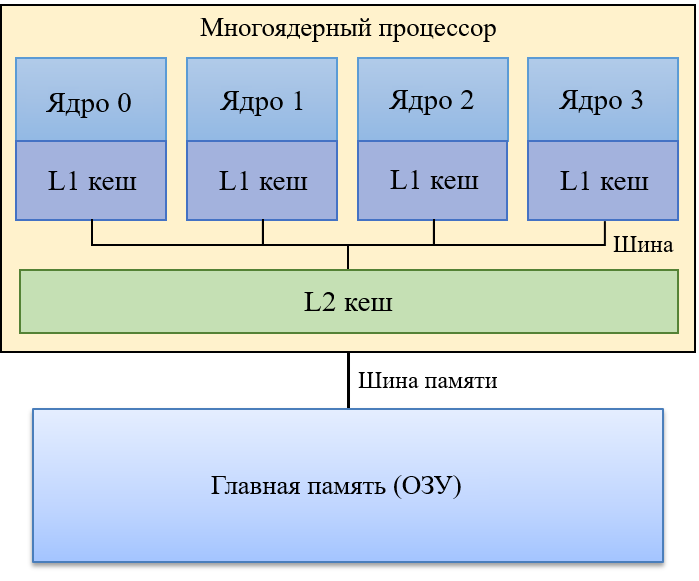
\includegraphics[width=95mm]{MulticoreCacheRU}
        \label{MulticoreCache}
    \end{figure}

    Каждое ядро процессора имеет собственный кеш инструкций и кеш данных, на которые для краткости
    ссылаются как на единый кеш 1-ого уровня. Остальные уровни кешей, как правило, являются объединёнными
    (для инструкций и данных).
    При промахе в кеш 1-ого уровня поиск данных происходит в кеше 2-ого уровня, при промахе
    в кеш 2-ого -- поиск в кеше 3-его (если таковой имеется), и так до тех пор, пока не произойдёт
    обращение в DDR память. (см. рис. \ref{MulticoreCache}).

    Как правило, кеш 2-ого уровня уникален для каждого ядра, хотя в некоторых гетерогенных системах
    кеш 2-ого уровня может использовать либо группой из 2-ух ядер в марках одного кластера, либо
    целиком всем кластером ядер (такое поведение характерно для современных энергоэффективных ядер).
    Кеш 3-его уровня всегда разделяется между всеми ядрами системы, как и системный кеш вместе с ОЗУ.

    ПЗУ, а также компоненты для долгосрочного хранения данных (диски, твёрдотельные накопители и др.)
    в данной работе рассматриваться не будут, под памятью будет иметься в виду только кеши процессора
    и ОЗУ.

\subsubsection{Латентность памяти и утилизация её пропускной способности} \label{lat_util_chapter}

    Начиная с этого момента и до коцна работы для краткости обозначения отношения величины
    затраченных тактов $cycles$ ядром процессора на исполнение количества инструкций $instrs$
    введём соотношение $cpi = cycles / instrs$.

    Для построения модели производительности ядра процессора, т.е. для правильного подсчёта утилизации
    ядра и наиболее энергоэффективного регулирования тактовых частот, важно учитывать не только
    структуру организации памяти в исследуемой системе, а также и динамические характеристики
    элементов такой системы. Наиболее важными характеристиками являются пропускная способность шин,
    соединяющих вычислительные подсистемы с подсистемами памяти, утилизация пропускной способности и
    латетность памяти -- промежуток времени между отправлением запроса на получение данных в память и
    между самим получением данных.

    Таким образом, кеши процессора и DDR память имеют свои собственные динамические характеристики,
    приведённые ранее. Как правило, низкие уровни кешей работают на той же тактовой частоте, что
    и само процессорное ядро, поэтому значение латентности таких кешей можно выразить через такты ядра
    процессора. Сложнее ситуация обстоит с более высокими уровнями кешей и DDR они имеют отдельные
    источники тактирования, значение латентности нельзя выразить через такты процессорного ядра,
    к тому же она зависит от утилизации пропускной способности шин, ведущих к этим элементам памяти,
    то есть от количества транзакций в единицу времени.

    Модель производительности ядра процессора требует учёта латентности памяти, поэтому
    необходимо рассмотреть существующие решения для её определения и/или возможного учёта в модели.

    Авторы статьи \cite{keramidas2010interval} предлагают 2 модели для учёта латентности памяти
    в рамках алгоритма регулирования тактовых частот. Первая модель разбивает такты ядра процессора
    на 2 компоненты: относящиеся к ожиданию транзакций памяти и относящиеся непосредственно к вычислительным
    блокам ядра процессора. Утверждается, что при изменении частоты ядра процессора изменяется только
    количество тактов, относящихся к памяти (тактовая частота которой независима от частоты ядра).
    На этом и основывается алгоритм регулирования частот, использующий перерасчёт времени
    исполнения через такты при различных частотах. Вторая модель является модификацией-улучшением
    первой модели: дополнительно предполагается, что в группе инструкций, которые обращаются в
    память подряд, следует учитывать только первую инструкцию в формуле для перерасчёта тактов,
    которые относятся к памяти, однако это требует наличие дополнительной информации на уровне кешей:
    среди всех промахов в кеши (т.е. обращений в следующий уровень памяти) следует учитывать только
    первые промахи среди группы промахов (промахов, находящихся на расстоянии порядка времени
    латентности обращения в вышележащие уровни памяти), что не поддерживается ни одним устройством
    на сегодняшний день.

    В работе также отмечается, что следует учитывать ROB в OoO процессорах: из тактов, относящихся к
    транзакциям памяти, следует вычесть ту часть тактов, которую тратит процессор на спекулятивное
    исполнение инструкций после инструкций-обращений в память.

    Подход использования аналитической формулы влияния утилизации пропускной способности памяти на
    её латентность рассматривается в статье \cite{clapp2015quantifying}: применяется
    метрика $cpi$, которая включает в себя слагаемые, связанные с тактами, потраченными
    на время ожидания транзакций-обращений в память. Авторы вводят понятие блокирующего фактора
    для латентности памяти: в зависимости от рабочей нагрузки при одинаковом количестве обращений в память
    влияние латентности на метрику ($cpi$) может меняться вплоть до десятка раз из-за параллельных
    обращений в память, что коррелирует с результатами работы \cite{keramidas2010interval}.
    При фиксированном блокирующем факторе значение $cpi$ зависит линейно от количества обращений
    в память в единицу инструкций.
    Таким образом, все рабочие нагрузки разделены на 2 вида: чувствительные к латентности (высокое
    значение блокирующего фактора) и чувствительные к пропускной способности (низкое значение
    блокирующего фактора).
    Однако данное исследование ограничивается рассмотрением обращений только в DDR память
    при фиксированных тактовых частотах всех устройств.

    Зависимость латентности памяти от утилизации пропускной способности представляет собой монотонную
    возрастающую функцию, которую можно положить константой при значениях утилизации, не сильно близкой
    к максимально возможной (\cite{david2011memory}), при приближении утилизации к своему максимуму
    значение латентности резко растёт.

    Таким образом, можно сделать основные выводы из существующих работ:
    \begin{enumerate}
        \item Чувствительность производительности к латентности памяти зависит от рабочей нагрузки и может
        быть очень низкой даже при большом количестве обращений в память (ОЗУ). Такая зависимость
        определяется уровнем параллелизма обращений в память.
        \item Латентность памяти является монотонной возрастающей функцией от утилизации пропускной
        способности, которую можно приближённо положить константой почти на всём интеравале утилизации;
        при стремлении утилизации к своему пределу происходит быстрый рост латентности до значений,
        на порядки превышающих значения при среднем уровне утилизации пропускной способности.
    \end{enumerate}

\subsection{Модель производительности ядра процессора}

    Главной характеристикой производительности процессора является количество инструкций,
    исполняемых в еденицу времени -- чем больше это значение, тем быстрее исполняется рабочая
    нагрузка (приложение). Причём заданное количество инструкций исполняется за разное количество
    процессорных тактов, которые, в свою очередь, обратно пропорциональны времени исполнения
    этих инструкций.

    Пусть за время $\tau$ ядро процессора непрерывно исполняло инструкции и исполнило $instrs$
    инструкций за $cycles$ тактов при заданной тактовой частоте процессора $freq_{cpu}$.
    Тогда, очевидно, выполняется следующее соотношение:

    \begin{equation} \label{cycles_base}
        cycles = \frac{freq_{cpu}}{\tau}
    \end{equation}

    На практике чаще всего используют такие величины как $cpi = cycles / instrs$ и
    $ipc = instrs / cycles$ в качестве меры эффективности ядра процессора: чем выше/ниже значение
    $ipc$/$cpi$, тем эффективнее работа ядра процессора. Однако кроме типа процессорного ядра
    на эти значения также влияют тактовая частота самого ядра и тактовые частоты остальных компонент
    системы. Например, при повышении частоты ядра процессора величина $ipc$ либо остаётся такой же,
    если отсутствуют инструкции, связанные с обращением высокие уровни кешей или ОЗУ, либо уменьшается.

    За время $\tau$ процессор часть тактов тратит на исполнение инструкций непосредственно на
    ядерных блоках (в том числе вычислительных), а оставшуюся часть на ожидание операций,
    связанных с обращением в память (в кеши или оперативную память): обозначим эти величины
    $cycles_{cpu}$ и $cycles_{mem}$, тогда справедливо

    \begin{equation}
        cpi = \frac{cycles}{instrs} = \frac{cycles_{cpu}}{instrs} + \frac{cycles_{mem}}{instrs}
    \end{equation}

    Важно отметить, что $\frac{cycles_{cpu}}{instrs}$ -- значение $cpi$, если бы все обращения
    в кеши и оперативную память занимали 0 тактов, т.е. обрабатывались бы бесконечно быстро, а значит
    эта величина ограничивается снизу возможностями ядра процессора. Обозначим данное соотношение
    как $cpi_{cpu} \equiv \frac{cycles_{cpu}}{instrs}$.

    В свою очередь величина $cycles_{mem}$ характеризуется только лишь компонентами памяти,
    не зависящими от конвейера ядра процессора. Пусть, например, имеется 2 уровня кешей
    и ОЗУ, тогда время доступа к определённому уровню кеша характеризуется величиной $cycles_{L_{i}}$,
    представляющую собой латентность кеша (время задержки обращения), выраженную в ядерных тактах,
    где $i$ -- номер уровня кеша.

    После обращения в кеш возможны 2 ситуации: либо попадание к кеш, либо промах и обращение в
    следующий уровень кеша или ОЗУ, если кеша высшего уровня не осталось.
    Время доступа к оперативной памяти обозначим $cycles_{ram}$.

    Выразим времена доступа через такты ядра процессора и латентности, и введя обозначение
    $time^{-1}_{*} = \alpha_{*}^{par} \cdot n_{*} \cdot \frac{lat_{*}}{freq_{*}}$, где
    $\alpha_{*}^{par}$ --
    коэффициент параллелизма обращений в соответствующую компоненту памяти (см. \ref{lat_util_chapter}),
    $n_{*}$ -- количество таких обращений за время $\tau$, $lat_{*}$ -- средняя латентность
    одного обращения, выраженное не в ядерных тактах, а в собственных тактах компоненты памяти, получим:

    \begin{equation}
        cycles_{mem} = \left( time^{-1}_{L_1} + time^{-1}_{L_2} + time^{-1}_{ram} \right) \cdot freq_{cpu},
    \end{equation}

    \begin{equation}
        cpi = cpi_{cpu} + cpi_{mem},
    \end{equation}

    \begin{equation}
        cpi_{mem} = \left( \frac{n_{L_1}}{instrs} \cdot \frac{\alpha_{L_1}^{par} \cdot lat_{L_1}}{freq_{L_1}} +
        \frac{n_{L_2}}{instrs} \cdot \frac{\alpha_{L_2}^{par} \cdot lat_{L_2}}{freq_{L_2}} +
        \frac{n_{ram}}{instrs} \cdot \frac{\alpha_{ram}^{par} \cdot lat_{ram}}{freq_{ram}} \right) \cdot freq_{cpu},
    \end{equation}

    Заметим, что из формулы следует, что повышение тактовой частоты ядра процессора ведёт к
    увеличению $cpi$ и уменьшению $ipc$, а повышение тактовых частот кешей и оперативной памяти,
    наоборот, ведёт к уменьшению $cpi$ и увеличению $ipc$.

    Чаще всего уровни кешей, наиболее близкие к процессорному ядру, имеют такой же источник
    тактирования, что и процессорное ядро, т.е. такие кеши оперируют на тех же тактовых частотах,
    что и само ядро. Например, кеш первого уровня (кеши инструкций и данных) всегда оперирует с
    тактовой частотой ядра процессора ($freq_{L_1} = freq_{cpu}$), а значит формулу можно упростить
    до более простой:

    \begin{equation}
        cpi = cpi_{cpu} + \alpha_{L_1}^{par} \cdot lat_{L_1} \cdot \frac{n_{L_1}}{instrs} +
        \left( \frac{n_{L_2}}{instrs} \cdot \frac{\alpha_{L_2}^{par} \cdot lat_{L_2}}{freq_{L_2}} +
        \frac{n_{ram}}{instrs} \cdot \frac{\alpha_{ram}^{par} \cdot lat_{ram}}{freq_{ram}} \right) \cdot freq_{cpu}.
    \end{equation}

    Заметим, что можно ввести обозначение,
    $cpi_{cpu}^{L_1} = cpi_{cpu} + \alpha_{L_1}^{par} \cdot lat_{L_1} \cdot \frac{n_{L_1}}{instrs}$,
    полностью убрав из рассмотрения параметры обращения в кеш 1-ого уровня.

    \begin{equation}
        cpi = cpi_{cpu}^{L_1} +
        \left( \frac{n_{L_2}}{instrs} \cdot \frac{\alpha_{L_2}^{par} \cdot lat_{L_2}}{freq_{L_2}} +
        \frac{n_{ram}}{instrs} \cdot \frac{\alpha_{ram}^{par} \cdot lat_{ram}}{freq_{ram}} \right) \cdot freq_{cpu}.
    \end{equation}

    Так как в данной работе не предполагается регулирование тактовых частот устройств памяти, то
    обозначим для удобства величины $C_{*} = lat_{*} / freq_{*}$; также обозначим
    $npi_{*} = \frac{n_{*}}{instrs}$:

    \begin{equation}
        cpi = cpi_{cpu}^{L_1} +
        \left( \alpha_{L_2}^{par} \cdot C_{L_2} \cdot npi_{L_2} +
               \alpha_{ram}^{par} \cdot C_{ram} \cdot npi_{ram} \right) \cdot freq_{cpu}.
    \end{equation}

    Заметим, что величины $C_{L_2}$ и $C_{ram}$ не являются константами в общем случае, так как
    имеют смысл латентности обращения в память, которая зависит утилизации пропускной способности
    шины, ведущей к соответствующей компоненте памяти (см. \ref{lat_util_chapter}).

    Латентность оперативной памяти определяется как текущим уровнем утилизации этой памяти
    (шины, ведущей к памяти), так и особенностями обращения к ней (например, в случае DDR
    памяти, где элементарными ячейками являются банки данных, состоящие из строк и столбцов,
    существует кеш строки, который значительно влияет на скорость обращения
    к ячейке памяти, т.е. локальность обращения к ячейкам DDR памяти очень важна).

    В качестве упрощения примем $\alpha_{L_2}^{par} = \alpha_{ram}^{par} = \alpha^{par}$ полагая,
    что коэффициенты параллелизма обращений в кеш последнего уровня (2-ого) и ОЗУ коррелируют.

    Финальная формула:

    \begin{equation} \label{cpi_formula}
        cpi = cpi_{cpu}^{L_1} + \alpha^{par} \cdot
        \left( C_{L_2} \cdot npi_{L_2} + C_{ram} \cdot npi_{ram} \right) \cdot freq_{cpu}.
    \end{equation}

    У описываемой модели есть ряд преимуществ, которые делают её лучше аналогичных моделей:
    \begin{enumerate}
        \item Явно введён коэффициент параллелизма обращений в память в $\alpha^{par}$, который можно
        регулировать динамически во время регулирования тактовой частоты ядра процессора.
        \item Такие величины, как $npi_{L_2}$ и $npi_{ram}$ можно получить в режиме реального времени
        практически во всех современных устройствах, в том числе в устройствах с архитектурой ARM64,
        которая используется в данной работе.
        \item Величины $C_{L_2}$ и $C_{ram}$ можно положить константами и вычислить заранее, так как
        в случае увеличения латентности памяти при приближении пропускной способности шин к максимальным
        значениям ответственность за увеличение этих коэффициентов неявно можно переложить на параметр
        $\alpha^{par}$, который уже предполагает дамическое регулирование.
        \item Величина $cpi_{cpu}^{L_1}$ не предполагает явного вычисления через другие формулы;
        достаточно знать все остальные коэффициенты, тогда эту величину можно найти по формуле
        \eqref{cpi_formula}, далее использовать её для оценки $cpi$ на других тактовых частотах.
        \item В случае физического ядра, разделённого на 2 виртуальных (так называемый
        SMT - Simultaneous multithreading), по-прежнему можно пользоваться формулой выше, т.к.
        становится неважно, как именно виртуальные ядра разделяют между собой процессорные блоки
        и как именно они взаимодействуют с кешом первого уровня -- эти аспекты учитываются
        в формуле в коэффициенте $cpi_{cpu}^{L_1}$ и не требуют дополнительных вычислений.
    \end{enumerate}

    Таким образом, для применения модели необходимо иметь:
    \begin{enumerate}
        \item Значения $C_{L_2}$ и $C_{ram}$, вычисленные заранее.
        \item Алгоритм регулирования $\alpha^{par}$.
        \item Возможность измерения величин $npi_{L_2}$ и $npi_{ram}$ в режиме реального времени.
    \end{enumerate}

% \subsection{Модель производительности применительно к архитектуре ARM}

%     [перепроверить всё, что идёт дальше]

%     Рассмотрим способ применения описанной выше модели в случае архитектуры ARM.
%     Для подсчёта значений $cycles$, $instrs$, $n_{L_2}$ и $n_{ram}$ можно ипользовать
%     следующие PMU счётчики процессора:
%     \begin{enumerate}
%         \item $CPU\_CYCLES$ -- количество затраченных процессорных циклов;
%         \item $INST\_RETIRED$ -- количество исполненных инструкций;
%         \item $L1I\_CACHE\_REFILL$ -- количество чтений инструкций (instruction fetches),
%         которые отсутствуют в кеше инструкций уровня L1 (промах в L1 кеш инструкций),
%         поэтому инструкции вынуждены читаться из кешей более высокого уровня.
%         Некешируемые промахи в кеш и операции синхронизации кешей не считаются;
%         \item $L1D\_CACHE\_REFILL$ -- количество чтений и записей данных (data loads and stores),
%         или операций обращений в таблицу страниц (page table walks), которые не смогли
%         найти нужную информацию в кеше данных уровня L1 (промах в L1 кеш данных),
%         поэтому данные вынуждены выгружаться из кешей более высокого уровня.
%         Некешируемые промахи в кеш и операции синхронизации кешей не считаются;
%         \item $L2D\_CACHE\_REFILL$ -- работает как сумма счётиков $L1D\_CACHE\_REFILL$ \\ и
%         $L1I\_CACHE\_REFILL$, но применительно к уровню кеша L2. В случае промаха в кеш дальнейшее
%         обращение может происходить не в кеш более высокого уровня, если таковой отсутствует,
%         а сразу в оперативную память.
%     \end{enumerate}

%     В счётчиках типа $\_CACHE\_REFILL$ существует очень важный нюанс, не оговорённый
%     в спецификациях PMU счётчиков компании ARM Ltd.,
%     но упоминаемый в иных документах: в платформах архитектуры ARM не существует PMU
%     счётчиков, которые считают промахи в кеши, вместо них используются счётчики, считающие
%     количество перезапонений кеш-линий (кешами более выского уровня ил оперативной памятью).
%     Возможна ситуация, когда один промах в кеш вызывает
%     несколько перезаполнений кеш-линий (например, если промах случился по адресу,
%     который пересекает 2 соседние кеш-линии), или наоборот: несколько промахов
%     в кеш могут быть разрешены благодаря одному перезаполнению кеш-линии.

%     Заметим, что чаще всего в современных мобильных системах на архитектуре ARM после последнего
%     уровня процессорного кеша располагают дополнительный кеш -- системный кеш (system cache),
%     который предназначен для периферийных устройств. Он может быть как больше по размеру, чем
%     последний уровень процессорного кеша, так и меньше. Наличия системного кеша ведёт к тому,
%     что для определения значения $n_{ram}$ недостаточно воспользоваться счётчиками, описанными
%     выше.

%     Единственный счётчик, который умеет считать количество промахов в кеш, является
%     $LL\_CACHE\_MISS\_RD$. Причиной тому является то, что кеш последнего уровня, как правило,
%     является системным кешом, который находится за пределами CPU на чипе. Данный счётчик считает
%     количество промахов, когда в результате данные берутся из оперативной памяти,
%     из другого чипа или из соседнего процессорного кластера с использованием технологии
%     Intercluster peering. Нас интересует только первый случай.

%     Согласно документации ARM, если счётчик $LL\_CACHE\_MISS\_RD$ не реализован, то есть
%     бит $EXTLLC$ в регистре $CPUECTLR$ выставлен в ноль, то значения $LL\_CACHE\_MISS\_RD$
%     будут совпадать со значениями $L2D\_CACHE\_REFILL$, так что в случае наличия
%     системного кеша такая ситуация может заметно ухудшить работу модели
%     (по-прежнему предполагается система из 2 уровней кеша и возможно системного кеша).

% \subsection{Модель производительности применительно к ядру Linux}

%     TBD

% \subsection{Реализация модели в планировщике ядра Linux}

%     TBD

\newpage
